% vim: set ts=4 sw=4 ai et tw=74:
\documentclass[12pt,a4paper,portuges]{style/myreport}
\usepackage[portuges]{babel}
\usepackage[utf8]{inputenc}

%%%%%%%%%%%%%%%%%%%%%%%%%%%%%%%%%%%%% DADOS DA CAPA DO RELATÓRIO %%%%%%%%%%%%%%%%%%%%%%%%%%%%%%%%%%%%%%5
\newcommand{\AnoLectivo}{Ano Lectivo de 2010/11}
\newcommand{\TituloProjecto}{Planeta XPTO, fase I}
\newcommand{\NomeDaCadeira}{Disciplina de Computação Gráfica}
\newcommand{\Curso}{Licenciatura em Engenharia Informática}

\newcommand{\PrimeiraListaNomes}{António Cascais, Fábio Costa, Gabriel Poça, José Teixeira, Miguel Palhas}

\newcommand{\PrimeiroElemento}{54744 - António Carlos Pinheiro Cascais}
\newcommand{\SegundoElemento}{54822 - Fábio Rafael Costa}
\newcommand{\TerceiroElemento}{56974 - Gabriel Gonçalves Poça}
\newcommand{\QuartoElemento}{54749 - José António Teixeira}
\newcommand{\QuintoElemento}{54767 - Miguel Branco Palhas}
%%%%%%%%%%%%%%%%%%%%%%%%%%%%%%%%%%%%% FIM %%%%%%%%%%%%%%%%%%%%%%%%%%%%%%%%%%%%%%5

\usepackage[T1]{fontenc}
\usepackage{a4wide}
\usepackage{txfonts}% use Arial && Times New Roman
\usepackage[pdftex]{color,graphicx}
\usepackage{fancyhdr}
\usepackage{fancyvrb}
\usepackage{acronym}
\usepackage{cite}
\usepackage{longtable}
\usepackage{datetime}
%\usepackage{amssymb}
\usepackage[pdfauthor={\PrimeiraListaNomes},%
            pdftitle={\{\TituloProjecto\}},%
            urlcolor=darkblue,%
            citecolor=darkblue,%
            filecolor=darkblue,%
            linkcolor=darkblue,%
            pdftex,colorlinks,a4paper]{hyperref}
\definecolor{darkblue}{rgb}{0,0,0.6}
%\definecolor{darkred}{rgb}{0.8,0,0}

%%%%%%%%%%%%%%%%%%%%%%%%%%%%%%%%%%%% PACOTES PARA ADICIONAR CODIGO FONTE %%%%%%%%%%%%%%%%%%%%%%%%%%%%%%%%%%%%%%
\usepackage{listings}
\usepackage{color}
\usepackage{textcomp}
\definecolor{listinggray}{gray}{0.9}
\definecolor{lbcolor}{rgb}{0.9,0.9,0.9}
\lstset{
	%backgroundcolor=\color{lbcolor},   					% COR DE FUNDO
	tabsize=4,
	rulecolor=,
	language=c,								% TIPO DE LINUGAGEM DE PROGRAMAÇÃO
        basicstyle=\scriptsize,
        upquote=true,
        aboveskip={1.5\baselineskip},
        columns=fixed,
        showstringspaces=false,
        extendedchars=true,
        breaklines=true,
        prebreak = \raisebox{0ex}[0ex][0ex]{\ensuremath{\hookleftarrow}},
        %frame=single,								% LINHA QUE CONTORNA O CODIGO
        showtabs=false,
        showspaces=false,
        showstringspaces=false,
        identifierstyle=\ttfamily,
        keywordstyle=\color[rgb]{0,0,1},
        commentstyle=\color[rgb]{0.133,0.545,0.133},
        stringstyle=\color[rgb]{0.627,0.126,0.941},
}

%%%%%%%%%%%%%%%%%         UTILIZAÇÃO:
%%%%%%%%%%%%
%%%%%%%%%%                  Imprimir com uma linha à volta do código
%%%%%%%%%%                       \begin{lstlisting}[frame=single]
%%%%%%%%%%
%%%%%%%%%%                  Imprimir normalmente:
%%%%%%%%%%                       \begin{lstlisting}
%%%%%%%%%%                           #include <SDL.h>
%%%%%%%%%%                       \end{lstlisting}
%%%%%%%%%%
%%%%%%%%%%                  Imprimir Ficheiro:
%%%%%%%%%%                       \lstinputlisting{filename.java}
%%%%%%%%%%%%
%%%%%%%%%%%%%%%%%%%%%%%%%%%%%%%%%%%% FIM %%%%%%%%%%%%%%%%%%%%%%%%%%%%%%%%%%%%%%

%%%%%%%%%%%%%%%%%%%%%%%%%%%%%%%%%%%% COMO ADICIONAR IMAGENS NO RELATÓRIO %%%%%%%%%%%%%%%%%%%%%%%%%%%%%%%%%%%%%%
%%%%%%%%%%%%%%
%                 \begin{figure}[here]
%                 \centering{\includegraphics[width=0.5\textwidth]{images/1imagem.png}}
%                 \caption{Prototipo de imagem}
%                 \label{fig:prototype}
%                 \end{figure}
%
%                 Please see Figure ~\ref{fig:prototype} for a prototype blah blah blah
%%%%%%%%%%%%%%
%%%%%%%%%%%%%%%%%%%%%%%%%%%%%%%%%%%% FIM %%%%%%%%%%%%%%%%%%%%%%%%%%%%%%%%%%%%%%

\pdfpagewidth=\paperwidth
\pdfpageheight=\paperheight

\renewcommand\familydefault{\sfdefault}% usar font sem serifas


%%%%%%%%%%%%%%%%%%%%%%%%%%%%%%%%%%%%% HEADER das paginas %%%%%%%%%%%%%%%%%%%%%%%%%
\pagestyle{fancy}

\fancyhead[LO,RE]{\footnotesize \slshape \rightmark}
\fancyhead[LE,RO]{\footnotesize \slshape \leftmark} 
%\fancyfoot{}
%\fancyfoot[LO,RE]{\thepage}

%%%%%%%%%%%%%%%%%%%%%%%%%%%%%%%%%%%% FIM %%%%%%%%%%%%%%%%%%%%%%%%%%%%%%%%%%%%%%

% definir acrónimos com itálico
%\renewcommand*{\acf}[1]{\acffont{\textit{\acl{#1}}~\acfsfont{(\acs{#1})}}}

\newtheorem{defin}{Definição}

%\pagestyle{fancy}
%\lhead{}
%\rhead{}

\newenvironment{comando}
{\medskip
\begin{tt}}
{\end{tt}
\medskip}

\parindent=0pt
\parskip=4pt

%
% Commands and environments
%
% vim: set ts=4 sw=4 ai et:

% insere uma imagem com legenda, por omissao com 12cm de largura
\newcommand{\image}[3][12cm]
{
    \begin{figure}[!h]
        \begin{center}
            \includegraphics[width=#1]{images/#2}
                \caption{#3}
                \label{fig:#2}
        \end{center}
    \end{figure}
    % force dump image queue here
    %\clearpage
}


\begin{document}

%% Capa Principal %%%%%%%%%%%%%%%%%%%%%%%%%%%%%%%%%%%%%%%%%%%%%%%%%%%%%%%
\thispagestyle{empty}

\setlength{\unitlength}{1cm}
\begin{picture}(0,0)

\put(14,0){\line(0,-1){24.5}}
\put(0,-12.2){\line(1,0){18}}
\put(0,-16.2){\line(1,0){18}}
\put(0,-12.2){\line(0,-1){4}}

\put(14.5,-3){
\includegraphics[height=2cm]{style/images/um}}
\put(14.5,-6){
\includegraphics[height=2cm]{style/images/eng}}
\put(14.5,-9){
\includegraphics[height=2cm]{style/images/di}}

\begin{minipage}[t]{16cm}
 
~

\addvspace{4cm}

Universidade do Minho

Conselho de Cursos de Engenharia

\Curso

\bigskip

{\Large \textbf{\NomeDaCadeira}}

\medskip

\AnoLectivo

\addvspace{7cm}

{\LARGE \ \TituloProjecto}

\addvspace{2.5cm}

\textbf{\PrimeiraListaNomes}

Grupo 26

\addvspace{0.5cm}

%
% Supervisão:  {\textless}{\textless}Orientador{\textgreater}{\textgreater}

\addvspace{2.5cm}

{\large \monthname, \newdateformat{dashdat}{\THEYEAR} \dashdat\today}

\end{minipage}
\end{picture}

\newpage

%% Segunda página %%%%%%%%%%%%%%%%%%%%%%%%%%%%%%%%%%%%%%%%%%%%%%%%%%%%%%%
\thispagestyle{empty}

\begin{flushright}
\begin{tabular}{|p{4cm}|p{4cm}|}
\hline
Data de Recepção & \\
\hline
Responsável & \\
\hline
Avaliação & \\
\hline
Observações & \\
& \\
& \\
\hline
\end{tabular}
\end{flushright}

~

\addvspace{8.4cm}

{\LARGE \textbf{ \TituloProjecto }}

\addvspace{2.5cm}

\textbf{\PrimeiroElemento}

\bigskip

\textbf{\SegundoElemento}

\bigskip

\textbf{\TerceiroElemento}

\bigskip

\textbf{\QuartoElemento}

\bigskip

\textbf{\QuintoElemento}

\addvspace{1.5cm}

{\large \monthname, \newdateformat{dashdate}{\THEYEAR} \dashdate\today}

\newpage

%% Página de dedicatória (opcional) %%%%%%%%%%%%%%%%%%%%%%%%%%%%%%%%%%%%%
%\thispagestyle{empty}

%{\textless}{\textless}Dedicatória{\textgreater}{\textgreater}

%\newpage

%% Resumo e Índices %%%%%%%%%%%%%%%%%%%%%%%%%%%%%%%%%%%%%%%%%%%%%%%%%%%%%
\pagenumbering{roman}
% vim: set ts=4 sw=4 ai et tw=74:
\chapter*{Resumo}
\addcontentsline{toc}{chapter}{Resumo} 


% indices
%\renewcommand{\contentsname}{Índice}
\tableofcontents
\addcontentsline{toc}{chapter}{\contentsname}

%\renewcommand{\listfigurename}{Índice de Figuras}
\listoffigures
\addcontentsline{toc}{section}{\listfigurename}

%%%%%%%%%%%%%%%%%%%%%%%%%%%%%%%%%%%% LISTA DE TABELAS %%%%%%%%%%%%%%%%%%%%%%%%%%%%%%%%
%\renewcommand{\listtablename}{Índice de Tabelas}
%\listoftables
%\addcontentsline{toc}{section}{\listtablename}

\newpage

%% Texto normal %%%%%%%%%%%%%%%%%%%%%%%%%%%%%%%%%%%%%%%%%%%%%%%%%%%%%%%%%
\pagenumbering{arabic}

%% TODO: uncomment chapters

\chapter{Introdução}
 %vim: set ts=4 sw=4 ai et tw=74:

%\addcontentsline{toc}{chapter}{Introdução}

%Falar do problema proposto
%Falar dos objectivos para esta primeira fase



Este projecto surge no âmbito da cadeira de Computação Gráfica, do curso de Engenharia Informática, no intuito de consulidar os conceitos objectivo da cadeira.

O projecto pela criação de um jogo, na linguagem C/C++ sobre a API OpenGl. O jogo consiste num mundo onde um jogador tem como objectivo alcançar o tesouro guardado num edifício, colocado no extremo do vale. Para tal deve recolher todas as chaves presentes no mundo. Como não podia faltar existem inimigos, neste caso, torres de proteção, que disparam sobre o jogador de forma a dicultar o processo.

Como suporte ao jogador existe um radar que detecta a distância à chave mais próximo dentro de um determinado alcance.





\newpage

\chapter{Considerações Inicias}
% 
%%terreno plano v
%%dois tipos de camara v
%%aleatoriedade e radar v
%%modelos importados e formato v
%%uma unidade em OpenGL corresponde a 0.1metros v

Existem algumas considerações iniciais a ter em conta.

São enunciadas várias dimensões,distâncias, em metros. Visto que em OpenGL não se realizam medições em metros foi necessário encontrar uma forma de relacionar as medidas do OpenGL com as medidas pedidas.
Assim, para que seja possível criar o jogo de acordo com as medidas pedidas no enunciado, considerámos que 1 metro corresponde a 4 unidades em OpenGL.

Quanto ao terreno, é pedido que seja plano com 4km quadrados de área. Utilizando texturas foi suficiente arranjar uma imagem de acordo com o pretendido e gerar o plano através dela.

Em termos de jogabilidade é necessária a implementação de dois modos de câmara: \textit{Third Person Shooter} (tps) e outra \textit{First Person Shooter} (fps).
Alternar entre estes dois modos é feito através de uma tecla pré-definida.

O radar não indica a direcção em que está a chave e tem um raio de acção limitado a 500 metros.

Por ultimo são necessário alguns modelos para as torres, chaves, herói, etc. Por opção, estes modelos são do formato \textit{.md2}. Adiante será desenvolvido este ponto e explicada esta escolha.


\newpage

\chapter{Ficheiro ini}


Um ponto relevante do projecto passa pelo ficheiro {\bf config.ini} . Neste documento estão todas as variáveis de uso frequente, ou melhor, todas as variáveis manipuláveis sem implicar recompilar o jogo, o que seria necessário para valores em \#define. Estes valores são "carregados"\ para o jogo quando necessário, mariotariamente no inicar do mesmo.

\-
\begin{center}
\begin{tabular} {l | p{10cm}}
\begin{lstlisting}
[game]
distance_factor		= 4
updates_per_second	= 60
anims_per_second	= 20
num_towers			= 15
num_keys			= 1
tower_range			= 1000
towers_min_distance = 500
\end{lstlisting} 
& 
Este é um exemplo de algumas configurações do jogo no documento {\bf config.ini}. \\
\end{tabular}
\end{center}

Este processo simplifica dois aspectos muito importantes. Para começar, possibilita a existência de um \emph{repositório} central com todos os valores usados ao longo do jogo. Por outro, facilita a alteração destes valores, o que ajuda bastante a efectuar pequenos ajustes no jogo sem ter a necessidade de recompilar o programa (processo que, como se constatou, tornou-se bastante longo á medida que o tamanho do código foi crescendo).

Eis de seguida um exemplo da utilidade desta classe, neste caso na criação da instância do jogador:

\begin{lstlisting}
Player::Player(const string &path) : Model_MD2(path) {
	state = GAME_ON;
	coords = new Vertex();
	coords->x = GLManager::distance(conf.rfloat("player:x"));
	coords->z = GLManager::distance(conf.rfloat("player:z"));
	coords->y = g_map->triangulateHeight(coords->x, coords->z);
	direction = new Vertex(0, 0, 1);
	ang_x = 0;
	ang_y = M_PI / 2;
	md2_rendermode = 0;

	speed_front = GLManager::convertFromKmH(conf.rfloat("player:speed_front"));
	speed_back = GLManager::convertFromKmH(conf.rfloat("player:speed_back"));
	speed_side = GLManager::convertFromKmH(conf.rfloat("player:speed_side"));
	speed_rotate_x = conf.rfloat("player:speed_rotate_x");
	speed_rotate_y = conf.rfloat("player:speed_rotate_y");


	anim = new Frame();
	anim->add_anim(MOVE_NONE, conf.rint("player:stop_frame"), conf.rint("player:stop_frame_end"));
	anim->add_anim(MOVE_WALK, conf.rint("player:walk_frame"), conf.rint("player:walk_frame_end"));
	anim->add_anim(MOVE_JUMP, conf.rint("player:jump_frame"), conf.rint("player:jump_frame_end"));

	jump_max = conf.rint("player:jump_max");
	isJumping = false;
	jump_time = 0;
	canJump = true;
	jump_cooldown = conf.rint("player:jump_cooldown");

	tower_colision_dist = conf.rint("player:tower_colision_dist");
	tree_colision_dist = conf.rint("player:tree_colision_dist");
}
\end{lstlisting}

Como se pode ver, esta classe depende fortemente de valores registados no ini, que são aqui lidos através das funções \textbf{conf.rint} e \textbf{conf.rfloat}, demonstrando assim a utilidade deste processo.


\newpage

\chapter{Modelos}
% vim: set ts=4 sw=4 ai et tw=74:

%\addcontentsline{toc}{section}{Desenho do Sistema}

%dizer que modelos importamos e em que formatos
%%dizer porque e que escolhemos esses formatos
%codigo

Carregar objectos no mundo, ou melhor, modelos para objectos, foi um dos grandes desafios. Tanto pela limitação da disponibilidade gratuita, como pelas limitações do carregamento dos modelos, do tipo \textit{obj}, que nos foram inicialmente apresentados.

Modelos \textit{obj} não são carregados com textura de origem, ou seja, o uso de texturas implicaria a implementação da funcionalidade. Em acréscimo nas limtações está a ausência de animações.
Neste contexto surgiu \textit{md2}, um formato original do motor do jogo quake.

\textit{MD2} é um formato abundante e bastante frequente existindo ainda uma ferramenta que facilita o carregamento para opengl, o {\bf md2loader}.

No jogo são carregados sobre a forma de modelos \textit{md2} os seguintes objectos:
\begin{itemize}
\item Player;
\item Torres;
\item Balas;
\item Chaves;
\item Edifício do Tesouro.
\end{itemize}


\newpage
\section{MD2 Loader}


Uma das ferramentas externas da qual o projecto faz uso é o {\bf md2loader}.

O md2loader é uma ferramenta de código aberto que facilmente adaptamos às nossas necessidades. Em palavras simples, existe uma classe denominada \textit{MD2Player} que permite carregar um modelo md2 e realizar operações simples como definir a escala ou render do modelo. Depois de conhecido o processo foi simples criar uma classe própria para trabalhar com a ferramenta.

\-

\begin{figure}[h]
\begin{center}
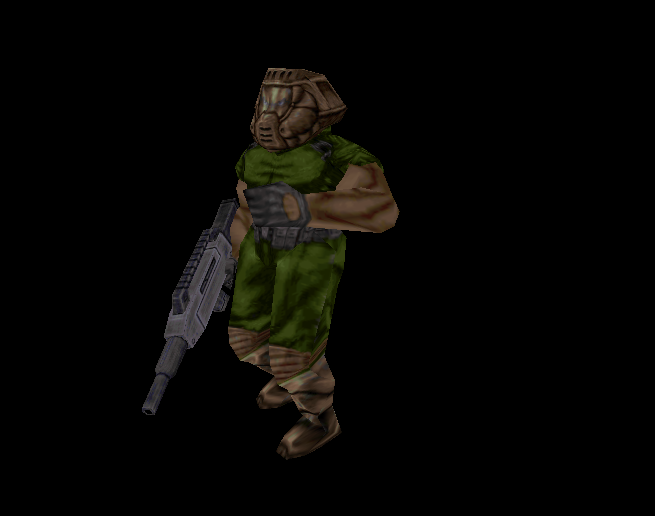
\includegraphics[width=0.5\textwidth]{images/md2loader.png}
\caption{Screenshot da ferramenta md2loader.}
\end{center}
\end{figure}




\newpage
\section{Player}

O player é aquele que se denomina ``herói'' do jogo. Ainda que nos seja permitido carregar qualquer modelo \textit{md2} optamos pela famosa figura dos jogos electrónicos, \textit{Sonic}.

Para controlar o player criamos uma classe, \textit{Player.cpp}.
Os modelos \textit{md2} utilizados suportam animações por frames. Assim, foi criada a classe Frame para gerir através da função \textbf{glutTimerFunc} o incremento das frames num intervalo fixo de tempo, configurável no ficheiro \textbf{config.ini}. Isto faz com que a cada intervalo, a frame actual seja incrementada, e quando o jogador está em movimento estas alternem ciclicamente, criando a ilusão de movimento.

\-
\begin{tabular} {l | p{10cm}}
\begin{lstlisting}
class Player : public Model_MD2 {
public:
	Frame *anim;
	float ang_x, ang_y;
	float speed_front, speed_back, speed_side;
	float speed_rotate_x, speed_rotate_y;
	float wall_dist;
	bool isJumping;
	int jump_time;
	int jump_max;
	bool canJump;
	int jump_cooldown;
	int tower_colision_dist;
	int tree_colision_dist;

	GameState state;

	Player(const std::string &path);

	void move(Vertex *new_coords);
	bool isMoving();
	void update();
	void render();

	float jumpOff(int off);

	static void inc_frame(int val);

	void calcColisions();
};
\end{lstlisting} 
&
Header da classe Player.cpp .\\
\end{tabular}

\subsection{Modos de Camera}
% vim: set ts=4 sw=4 ai et tw=74:

%\addcontentsline{toc}{chapter}{Lista de Acrónimos}

%Falar dos dois tipos de camaras
%Tecnicas para a implementaçao destes tipos
%como mudar entre as camaras
%codigo

A câmera é posicionada no mundo relativamente ao posicionamento e direcção do jogador. são implementados dois modos de visualização.
Em termos práticos, o cálculo da posição da câmara consiste em cálculos a partir dos vectores de posição e direcção do jogador, com alguns ajustes para um melhor posicionamento. Isto depende, obviamente do tipo de câmara utilizada:

\begin{description}
\item[Terceira Pessoa] Câmara colocada atrás do modelo ligeiramente acima e com a direcção do modelo. Ao vector de posição do jogador, é subtraido o seu próprio vector de direcção multiplicado por um factor de distância, para colocar a câmara nas costas do jogador. Há ainda um ajuste na coordenada Y para câmara ficar ligeiramente acima do jogador e ser possivel ver o que está para a frente deste. É também feito um teste para impedir que a câmara se posicione abaixo do nivel do terreno.
\item[Primeira Pessoa] Câmara colocada em frente ao modelo com a direcção do modelo. O método de calculo é semelhante ao anterior, apenas muda a equaçao, para posicionar a câmara á frente do jogador, em vez de nas suas costas.
\end{description}

Para ficar mais claro, eis o código de cálculo da posição da câmara:

\begin{lstlisting}[caption=Função de posicionamento da câmara]
void Camera::placeCamera() {
	Vertex* pos = g_player->coords;
	Vertex* dir = g_player->direction;

	glLoadIdentity();

	int cam_mode = InputManager::getOpState(CAMERA_MODE);

	if (cam_mode == KEY_OFF) {
		int tps_off = conf.rint("camera:tps_off");
		int tps_y_off = conf.rint("camera:tps_y_off");
		int tps_dir_y_off = conf.rint("camera:tps_dir_y_off");

		camPos->x = pos->x - tps_off * dir->x;
		camPos->z = pos->z - tps_off * dir->z;
		camPos->y = max(pos->y - tps_off * dir->y + tps_y_off, g_map->triangulateHeight(camPos->x, camPos->z) + terrain_offset);

		camDir->x = pos->x;
		camDir->y = pos->y + tps_dir_y_off;
		camDir->z = pos->z;
	} else {
		int fps_off = conf.rint("camera:fps_off");
		int fps_y_off = conf.rint("camera:fps_y_off");
		int fps_dir_y_off = conf.rint("camera:fps_dir_y_off");

		camPos->x = pos->x + fps_off * dir->x;
		camPos->z = pos->z + fps_off * dir->x;
		camPos->y = max(pos->y + fps_y_off, g_map->triangulateHeight(camPos->x, camPos->z));

		camDir->x = pos->x + (fps_off + 1) * dir->x;
		camDir->y = pos->y + dir->y + fps_dir_y_off;
		camDir->z = pos->z + (fps_off + 1) * dir->z;
	}


	gluLookAt(camPos->x, camPos->y, camPos->z,
		camDir->x, camDir->y, camDir->z,
		0, 1, 0);
}

\end{lstlisting} 

O código começa por saber as coordenadas e direcção do jogador, e conforme o tipo de câmara seleccionado (a câmara pode ser alternada pela tecla 'C'), calcula as posições da câmara, terminando então com a chamada ao \textbf{gluLookAt}.

\newpage
\section{Torres e Keys}
Para a gestão das torres e das existem duas classes, \textit{Towers.cpp} e \textit{Keys.cpp} respectivamente.

\-
\begin{center}
\begin{tabular} {l | p{10cm}}
\begin{lstlisting}[caption=Cabeçalho da classe Keys]
class Keys {
public:
    int num_keys, catched_count;
    float catch_dist;
    Key **keys;

    Keys();

    void render();
    void update();
    int get_closest_distance();
};
\end{lstlisting} 
& 
Header da classe Keys.cpp .
\end{tabular}
\end{center}
\-
Como se pode ver a classe keys é constituida por um array de instâncias da classe \emph{Key}, um numero de chaves (\emph{num\_keys}) que se encontra no documento config.ini e o numero de chaves apanhadas pela jogador (\emph{catched\_count}).
Existe ainda um método de update, que actualiza o modelo das chaves, determina se uma chave foi ou não apanhada, um método de render, que desenha as torres no mundo e por ultimo um método que calcula a distancia da chave que se encontra a menor distancia do jogador, inferior a 500 metros.

Para as torres o conceito é o mesmo, com a excepção do \emph{catched\_count} e do método \emph{get\_closest\_distance}.
No entanto as torres têm a caracteristaca de rodar na direcção do jogador quando este se encontra no seu alcance.

Na inicialização do jogo, são calculadas posições aleatórias para as chaves e torres. Estas posições têm em conta que uma torre ou chave nunca deverá ficar a menos de uma determinada distância (definida no ficheiro ini) de outra chave ou torre, evitando assim por exemplo, que uma chave fique escondida dentro do modelo de uma torre.

O algoritmo de cálculo da {\bf distancia entre dois modelos} é simples. Tendo as coordenadas do dos modelos temos:

\begin{center}
\begin{math}
Player => (a1,b1)
\end{math}
,
\begin{math}
Tower => (a2,b2)
\end{math}

\begin{equation}
Distancia = \sqrt{((a1-a2)^2+(b1-b2)^2)}
\end{equation}
\end{center}


\subsection{Angulo de orientação das Torres}

O angulo de orientação das torres para o player pode ser determinado fazendo uso do produto escalar entre dois vectores, a direção do player para a torre e o vector unitário (1,0,0). Sabemos que

\-
\begin{center}
\begin{math}
Player => (a_1,a_2)
\end{math}
,
\begin{math}
Tower => (b_1,b_2)
\end{math}

\begin{equation}
produto escalar = a_1*b_1 + a_2*b_2
\end{equation}
\begin{equation}
produto escalar = direccao * unitario * cos x
\end{equation}
\end{center}

Como tal, orientado em função do angulo \emph{x} temos:

\begin{equation}
x = acos( (a_1*b_1 + a_2*b_2 ) / direccao * unitario * cos x )
\end{equation}


Este angulo é a orientação que uma torre deve assumir para se orientar para um player, está claro, quando a distância é inferior ao alcance da torre.






\newpage

\chapter{Radar}
O radar apresenta a distância à chave mais próxima num limite de 500 metros, valor que pode facilmente ser editado no ficheiro \textbf{config.ini}.
A informação é mostrada textualmente no ecrã. Quando todas as chaves são apanhadas, essa informação é reflectida no radar, que indica ao jogador que deve procurar o final.

\begin{figure}[here]
                 \centering{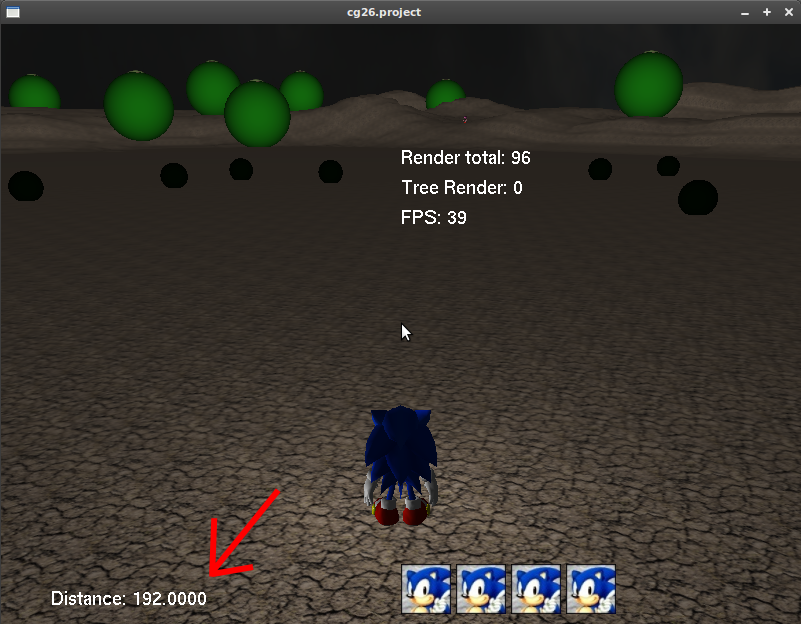
\includegraphics[width=0.9\textwidth]{images/radar.png}}
                 \caption{Radar.}
                 \label{fig:prototype}
\end{figure}


\newpage

\chapter{Input}
O input é tratado através da classe InputManager. Esta classe mantém uma estrutura com o estado actual de todas as teclas utilizadas no jogo, bem como informação sobre as coordenadas e movimento do rato. Os eventos de pressionar ou libertar uma tecla apenas accionam um método que altera o estado da tecla correspondente na estrutura.

Assim, em qualquer ponto do código, é possivel saber o estado de uma tecla (pressionada ou não), e consoante essa flag, executar uma determinada acção. Esta estruturação permite uma gestão mais flexivel do input do que aquela utilizada nas aulas práticas, em que a função de gestão do input executava as próprias acções. Isto fazia com que a interacção fosse mais limitada, não sendo considerada a utilização de várias teclas ao mesmo tempo. Essa funcionalidade já é obtida por uma estrutura como a classe aqui utilizada.

Foi assim possivel implementar facilmente a utilização de várias teclas para ligar/desligar determinadas opções durante o decorrer do jogo:
\begin{itemize}
\item[C] Alternar entre os dois modos de câmera;
\item[M] Ligar/Desligar a música;
\item[N] Ligar/Desligar os restantes sons;
\item[F1] Activar o modo GL\_LINES da função {\textbf glPolygonMode} (para efeitos de Debug);
\item[F2] Desactivar o modo GL\_LINES;
\item[P] Activar/Desactivar o Profiling
\item[W,A,S,D] Movimentar o jogador pelo terreno;
\item[Espaço] Saltar;
\item[Rato] O movimento do rato traduz-se em movimento da câmara na direcção correspondente, e também da orientação do jogador no terreno;
\end{itemize}


\newpage

\chapter{Extras}
\section{SkyBox}

Um pequeno extra que permite criar um ambiente à volta do mundo, no nosso caso, acrescentar um céu ao mundo. SkyBox consiste em desenhar um cubo centrado no player cujas faces estejam no limiar da visão do mesmo, e por dentro colocar uma textura, por face, onde os lados se completem.

\-

\begin{figure}[h]
\begin{center}
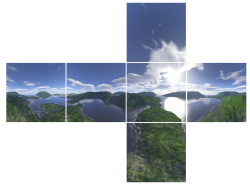
\includegraphics[width=0.5\textwidth]{images/skybox.png}
\caption{Exemplo de um textura para skybox.}
\end{center}
\end{figure}
\newpage
\section{Sound}
Digamos que a experiência agradavel de um jogo nao esta apenas na visão. O som é também importante. Como tal acrescentamos este extra ao jogo, conseguindo-o através da biblioteca openAL. Na primeira etapa entregamos apenas alguns sons e uma musica  de fundo, nesta etapa, munidos dos clássicos sons da famosa personagem \textit{Super Mario}, fazemos o jogo ganhar outro significado, existe assim som para o salto, para a perda de vida, para o "ganhar o jogo", para o "perder o jogo" e de fundo.


\chapter{Notas Conclusivas}
Nesta primeira fase concluimos todos os objectivos do enunciado e implementámos ainda alguns extras. Terminamos assim com um jogador sobre um mundo plano, torres com movimento, chaves e um edificio do tesouro, e som e animações como extra. Para a próxima etapa contamos com carregar um mundo através de um mapa de alturas, implementar os disparos da torre e aplicar algumas tecnicas de computação gráfica para optimizar o trabalho.

\chapter*{Bibliografia}
% vim: set ts=4 sw=4 ai et tw=74:

\addcontentsline{toc}{chapter}{Bibliografia}

Stephen L. Nelson, Pat Coleman, Kaarin Dolliver, \textit{Effective Executives Guide to Microsoft Project 2000}, Redmond Technology Press, 2000, ISBN 1-931150-16-8\\ \\

M. Fowler. \textit{UML Distilled}, Third Edition. Addison-Wesley, 2004, ISBN 0-321-19368-7\\ \\

Sommerville, Ian, \textit{Engenharia de Software}, 8ª Edição, 2007, ISBN: 9788588639287

%Martins, Mário F. \textit{ JAVA5 e Programação por Objectos}, FCA - Editora Informática, 2006, ISBN 9789727225484\\ \\


\chapter*{Referências}
\textbf{Livros}
\begin{itemize}
\item{"OpenGL Programming Guide", Woo, Neider, Davis and Schneider, Addison Wesley}
\end{itemize}


\textbf{Sites}
\begin{itemize}
\item{www.lighthouse3d.com, acedido em Maio 2010}
\item{www.opengl.org, acedido em Maio 2010}
\item{www.gamasutra.com, acedido em Maio 2010}
\end{itemize}



%\input{7acron}

\appendix
\chapter{Código fonte}
\section*{Model.h}
\lstinputlisting{../Model.h}
\pagebreak
\section*{GLManager.cpp}
\lstinputlisting{../GLManager.cpp}
\pagebreak
\section*{Config.cpp}
\lstinputlisting{../Config.cpp}
\pagebreak
\section*{SkyBox.cpp}
\lstinputlisting{../SkyBox.cpp}
\pagebreak
\section*{Towers.h}
\lstinputlisting{../Towers.h}
\pagebreak
\section*{Bullet.h}
\lstinputlisting{../Bullet.h}
\pagebreak
\section*{Vertex.h}
\lstinputlisting{../Vertex.h}
\pagebreak
\section*{Key.h}
\lstinputlisting{../Key.h}
\pagebreak
\section*{Model\_MD2.h}
\lstinputlisting{../Model_MD2.h}
\pagebreak
\section*{Sound.h}
\lstinputlisting{../Sound.h}
\pagebreak
\section*{Keys.cpp}
\lstinputlisting{../Keys.cpp}
\pagebreak
\section*{Tower.h}
\lstinputlisting{../Tower.h}
\pagebreak
\section*{Profiling.h}
\lstinputlisting{../Profiling.h}
\pagebreak
\section*{Lifes.h}
\lstinputlisting{../Lifes.h}
\pagebreak
\section*{Player.cpp}
\lstinputlisting{../Player.cpp}
\pagebreak
\section*{Trees.h}
\lstinputlisting{../Trees.h}
\pagebreak
\section*{InputManager.cpp}
\lstinputlisting{../InputManager.cpp}
\pagebreak
\section*{Towers.cpp}
\lstinputlisting{../Towers.cpp}
\pagebreak
\section*{Plane.h}
\lstinputlisting{../Plane.h}
\pagebreak
\section*{Map.cpp}
\lstinputlisting{../Map.cpp}
\pagebreak
\section*{Frustum.cpp}
\lstinputlisting{../Frustum.cpp}
\pagebreak
\section*{Map.h}
\lstinputlisting{../Map.h}
\pagebreak
\section*{SkyBox.h}
\lstinputlisting{../SkyBox.h}
\pagebreak
\section*{InputManager.h}
\lstinputlisting{../InputManager.h}
\pagebreak
\section*{Toilet.h}
\lstinputlisting{../Toilet.h}
\pagebreak
\section*{Bullet.cpp}
\lstinputlisting{../Bullet.cpp}
\pagebreak
\section*{Radar.cpp}
\lstinputlisting{../Radar.cpp}
\pagebreak
\section*{Lighting.h}
\lstinputlisting{../Lighting.h}
\pagebreak
\section*{Lifes.cpp}
\lstinputlisting{../Lifes.cpp}
\pagebreak
\section*{ChangeMode.h}
\lstinputlisting{../ChangeMode.h}
\pagebreak
\section*{Lighting.cpp}
\lstinputlisting{../Lighting.cpp}
\pagebreak
\section*{Rainbow.h}
\lstinputlisting{../Rainbow.h}
\pagebreak
\section*{Player.h}
\lstinputlisting{../Player.h}
\pagebreak
\section*{Frame.h}
\lstinputlisting{../Frame.h}
\pagebreak
\section*{Trees.cpp}
\lstinputlisting{../Trees.cpp}
\pagebreak
\section*{Config.h}
\lstinputlisting{../Config.h}
\pagebreak
\section*{Textures.cpp}
\lstinputlisting{../Textures.cpp}
\pagebreak
\section*{externs.h}
\lstinputlisting{../externs.h}
\pagebreak
\section*{Rainbow.cpp}
\lstinputlisting{../Rainbow.cpp}
\pagebreak
\section*{Bullets.h}
\lstinputlisting{../Bullets.h}
\pagebreak
\section*{Textures.h}
\lstinputlisting{../Textures.h}
\pagebreak
\section*{Sound.cpp}
\lstinputlisting{../Sound.cpp}
\pagebreak
\section*{Radar.h}
\lstinputlisting{../Radar.h}
\pagebreak
\section*{Tree.cpp}
\lstinputlisting{../Tree.cpp}
\pagebreak
\section*{Key.cpp}
\lstinputlisting{../Key.cpp}
\pagebreak
\section*{Model\_MD2.cpp}
\lstinputlisting{../Model_MD2.cpp}
\pagebreak
\section*{Model.cpp}
\lstinputlisting{../Model.cpp}
\pagebreak
\section*{Tree.h}
\lstinputlisting{../Tree.h}
\pagebreak
\section*{GLManager.h}
\lstinputlisting{../GLManager.h}
\pagebreak
\section*{Camera.cpp}
\lstinputlisting{../Camera.cpp}
\pagebreak
\section*{Camera.h}
\lstinputlisting{../Camera.h}
\pagebreak
\section*{Frustum.h}
\lstinputlisting{../Frustum.h}
\pagebreak
\section*{Toilet.cpp}
\lstinputlisting{../Toilet.cpp}
\pagebreak
\section*{ChangeMode.cpp}
\lstinputlisting{../ChangeMode.cpp}
\pagebreak
\section*{Profiling.cpp}
\lstinputlisting{../Profiling.cpp}
\pagebreak
\section*{Plane.cpp}
\lstinputlisting{../Plane.cpp}
\pagebreak
\section*{Keys.h}
\lstinputlisting{../Keys.h}
\pagebreak
\section*{Main.cpp}
\lstinputlisting{../Main.cpp}
\pagebreak
\section*{Tower.cpp}
\lstinputlisting{../Tower.cpp}
\pagebreak
\section*{Bullets.cpp}
\lstinputlisting{../Bullets.cpp}
\pagebreak
\section*{Vertex.cpp}
\lstinputlisting{../Vertex.cpp}
\pagebreak
\section*{Frame.cpp}
\lstinputlisting{../Frame.cpp}
\pagebreak

%\input{8anexos}

\end{document}
